\subsection{Schätzverfahren}
\label{sec_curveFit}
In diesem Abschnitt wird das implementierte Schätzverfahren erläutert. Das Verfahren nutzt die Ergebnisse der Bilderkennung und versucht mithilfe der Regression ein Polynom $f$ zweiten Grades durch alle erkannten Punkte unter Betrachtung ihrer Orientierung zu fitten. Da von geringen Krümmungsgraden der Objekte ausgegangen wird bildet eine Polynom zweiten Grades ein gutes Modell der Objekte. Mit einer Geraden wäre es nicht möglich auch nur den leichtesten Krümmungsgrad angemessen abzubilden. Polynome höheren Grades haben in diesem Anwendungsfall das Problem leicht zu \textit{kurvig} zu extrapolieren. Im Bereich der detektierten Punkte können auch solche Polynome gute Ergebnisse liefern, im Bereich danach jedoch sehr leicht mit starker Krümmung abfallen. Außerdem wäre der Parameterraum für die Regression mit jedem höheren Grad erhöht, ohne einen Mehrwert zu bieten.\\
Der Ansatz basiert auf dem \textit{Least-Squares} Verfahren\cite{simon2006optimal}, wobei versucht wird, die Gleichung \ref{lsq} zu minimieren.
$x_i$ und $y_i$ sind hierbei die Koordinaten der erkannten Punkte. Es wird über alle Punkte der quadratische Fehler vom Funktionswert für ein $x$ zu gegebenen Modellparametern $p$ zum $y$ aus der Bilderkennung summiert. $f(p,x)$ ist eine beliebige Funktion, die $x$ in Abhängigkeit von $p$ auf eine reelle Zahl abbildet.\\
\begin{ownequation}[H]
\begin{equation}
err = \sum_{i}(f(p,x_i)-y_i)^2
\end{equation}
\caption[Least-Squares-Ansatz]{Least-Squares-Ansatz. $x_i$ und $y_i$ sind die erkannten Objektpositionen.}
\label{lsq}
\end{ownequation}
Über die Zeit gesehen wird die Menge an detektierten Punkten immer größer. Da das Ziel des Verfahrens die Vorhersage des Objektverlaufs ist, ist eine gute Extrapolation wichtiger als das richtige Abbilden aller Punkte der Vergangenheit. Für die Extrapolation ist anzunehmen, dass neuere Punkte für den Verlauf wichtiger sind als ältere. Aus diesem Grund werden die Punkte über die Zeit exponentiell aufsteigend gewichtet. Somit erhalten aktuelle Punkte einen höheren Stellenwert als ältere, ohne jedoch alte Punkte komplett zu verwerfen.\\
Um diese Anforderungen umzusetzen wird eine Erweiterung des \textit{Least-Squares} verwendet, den \textit{Weighted-Least-Squares}[Gleichung \ref{wlsq}]\\
\begin{ownequation}[H]
\begin{equation}
err = \sum_{i}w_i \cdot (f(p,x_i)-y_i)^2
\end{equation}
\caption[Weighted-Least-Squares-Verfahren]{Weighted-Least-Squares Verfahren. Erweitert das Least-Squares Verfahren um eine Gewichtung der Punkte.}
\label{wlsq}
\end{ownequation}
\newpage
Das \textit{Weighted-Least-Squares} Verfahren bietet eine gute Grundlage für die Regression. Es bleiben jedoch noch einige Probleme, die das Verfahren in der Form nicht lösen kann.
\begin{enumerate}
\item Beachtung der Orientierung erkannter Punkte
\item Bedingungen für die Kurve (z.B. maximale Steigung)
\item Schätzungen für Punktverläufe, die sich nicht durch ein einzelnes Polynom darstellen lassen
\end{enumerate}

Zum Lösen der ersten zwei Probleme bietet die \matlab -Funktion \textit{fmincon}\footnote{https://de.mathworks.com/help/optim/ug/fmincon.html} aus der Optimization Toolbox eine geeignete Lösung. Die Funktion bietet die Möglichkeit eine Funktion $F(p)$ zu minimieren, wobei mit $c(p) \leq 0$ eine Bedingung erfüllt werden muss. Die Funktion $c(p,x_i)$ [Gleichung \ref{constraint}] berechnet über den Funktionsverlauf von $f(p,x)$ mithilfe der Ableitung $f'(p,x)$ die Steigung in jedem Punkt $x_i$. Da \textit{fmincon} prüft, ob die Bedingungsfunktion kleiner 0 ist wird von der Steigung ein Maximalwert ($max_{slope}$) abgezogen (\textit{Erfüllt 2.}).\\
\begin{ownequation}[H]
\begin{equation}
c(p,x_i) = f'(p,x_i)-max_{slope}
\end{equation}
\caption[Funktion zum Überprüfen ob die Steigung einen Maximalwert nicht übersteigt.]{Funktion zum Überprüfen, ob die Steigung einen Maximalwert nicht übersteigt. $max_{slope}$ gibt die maximal erlaubte Steigung des Polynoms an, die mit der Ableitung der Funktion überprüft wird.}
\label{constraint}
\end{ownequation}
Die Funktion $F(p)$ wird als $F(p,x,y,s,w,n,m,tau)$ [Gleichung \ref{minimizeFunction}] definiert, wobei $x$ und $y$ erneut die Punkte der Bilderkennung darstellen, $s$ die erkannte Orientierung im Punkt und $w$ das Gewicht darstellt. Die Funktion $F$ besteht aus einer Linearkombination der Funktionen $g$ und $h$, wobei $g$ den summierten Fehler der Position [Gleichung \ref{posError}] ($x$,$y$ Koordinaten) und $h$ den summierten Fehler der Orientierung [Gleichung \ref{orienError}] mithilfe des \textit{Weighted-Least-Squares} Verfahren berechnen (\textit{Erfüllt 1.}). $n$ und $m$ gewichten, wie stark die einzelnen Fehlerarten (Position und Orientierung) in den Gesamtfehler für die gegebenen Funktionsparameter $p$ eingehen.\\
Um die erhaltenen Polynome einschränken zu können, wurde $F$ noch gemäß der \textit{Tikhonov Regularisierung} \cite{kaipio2006statistical} angepasst. Durch die \textit{Tikhonov-Regularisierung} können wenig gekrümmte Kurven bevorzugt werden, was für einen ruhigeren Fahrtverlauf sorgen kann.
\begin{ownequation}[H]
\begin{equation}
\label{minimizeFunction}
F(p) = F(p,x,y,s,w,n,m,tau) = n \cdot g(p,x,y,w) + m \cdot h(p,x,s,w) + tau \cdot p
\end{equation}
\begin{equation}
\label{posError}
g(p,x,y,w) = \sum_{i} w_i \cdot (f(p,x_i)-y_i)^2
\end{equation}
\begin{equation}
\label{orienError}
h(p,x,s,w) = \sum_{i} w_i \cdot (f'(p,x_i)-s_i)^2
\end{equation}
\caption[Definition der Funktion F, die im Schätzverfahren minimiert wird.]{Zusammensetzung der Funktion F, die minimiert wird. In (\ref{posError}) wird der \textit{Weighted-Least-Squares} auf den Fehler der Position und in (\ref{orienError}) auf den Fehler der Steigung angewendet.}
\label{F-function}
\end{ownequation}
\newpage
Um das Problem 3. zu lösen, betrachten wir Abbildung \ref{prob3}. Das Objekt ist hierbei so gelegen, dass das Polynom nur sehr schlecht durch die Daten gelegt werden kann und außerdem ein Teilabschnitt annähernd parallel zur Y-Achse verläuft. Der letzte Fall ist zu beachten, da ein solcher Verlauf durch eine unendliche Steigung im Polynom abgebildet werden müsste.\\
Als Lösung für dieses Problem wird ein alternatives Weltkoordinatensystem eingeführt. Dieses unterscheidet sich durch eine \gls{transform} vom echten Weltkoordinatensystem. In Abbildung \ref{prob3solved} ist zu sehen, wie durch eine \gls{transform} ein weitaus besseres Polynom für die gleichen Punkte gefunden werden kann.\\
\begin{figure}[H]
\centering
\begin{tabular}{cc}
\subfloat[Die detektierten Punkte sind so gelegen, dass das Polynom nur sehr schlecht durch die Daten gelegt werden kann.]{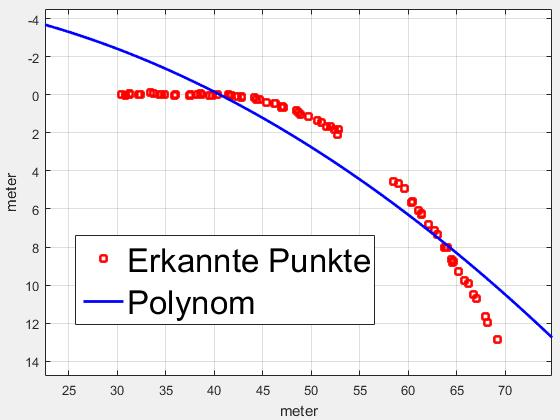
\includegraphics[scale=0.55,width=0.45\textwidth]{curveFitting/bevoreTrans.jpg}\label{prob3}}&
\subfloat[Durch die Transformation wird ein deutlich besseres Polynom gefunden.]{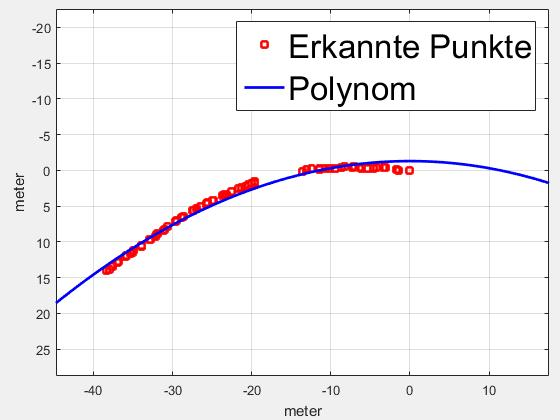
\includegraphics[scale=0.55,width=0.45\textwidth]{curveFitting/afterTrans.jpg}\label{prob3solved}}
\end{tabular}
\caption[Transformation in alternatives Koordinatensystem]{Eine Transformation der detektierten Punkte in das alternative Koordinatensystem, um ein besseres Polynom bestimmen zu können. Das Polynom in \textit{a)} übersteigt den Fehlerschwellenwert und löst damit die Transformation aus.}
\label{figAlterCoords}
\end{figure}
Nach jeder Regression wird das berechnete Polynom in den aktuellsten Punkten getestet. Sollte dabei ein gewisser Fehlerschwellenwert überschritten werden, wird eine neue \gls{transform} berechnet (vgl. Listing \ref{transPseudo}). Diese neue Transformation besteht aus einer Translation zum Punkt mit dem größten $x$-Wert und einer Rotation um die durchschnittliche Ausrichtung der neuesten Punkte. Neben der Transformationsmatrix wird auch die Inverse der Matrix gespeichert, die für die Wegpunktberechnung [Kapitel \ref{sec_waypoint}] wichtig ist. Da die Transformation ausgelöst wird, sobald das Polynom in den neuesten Punkten einen zu großen Fehler ergibt, werden nach dem Speichern der Matrizen alle Punkte, bis auf die neuesten, verworfen, um ein potentiell besseres Polynom für die Extrapolation zu ermöglichen. Die \textit{aktuellsten} Punkte wurden im Rahmen dieser Arbeit auf konstant 10 Punkte gesetzt. Bei einer größeren Anzahl an Punkten, die nach einer neuen Transformation nicht verworfen werden, konnte oftmals kein neues Polynom gefunden werden, dass die maximale Fehlerschwelle wieder unterschreitet.\\
Sobald eine beschriebene \gls{transform} gespeichert wurde, werden alle Punkte vor der Regression in das alternative Koordinatensystem transformiert. Durch diese Transformation sind die erkannten Punkte entlang der X-Achse gelegen und somit ist es möglich, stets ein geeignetes Polynom für die Punkte zu finden. Durch die Translation liegen die Punkte stets nah am Ursprung, was den Parameterraum für die Regression verringert und somit zu schnelleren Ergebnissen führt.\label{alterWorldCoords}
\begin{lstlisting}[language=Matlab,caption=Pseudocode des Schätzverfahrens,label=transPseudo]
function polynomFit(points,maxError)
	actualTransform = loadActualTransformation();
	points_T = transformPoints(points,actualTransform);
	
	polynom = regression(points_T);
	error = calculateError(points_T,polynom);
	if (error >= maxError)
		translation = findGreatestXValue(points_T);
		rotation = averageDirectionOfLastPoints(points_T);
		newTransform = createTransMatrix(-translation,-rotation) * actualTransform;
		saveNewTransform();
	end
end
\end{lstlisting}
In Listing \ref{transPseudo} ist das Schätzverfahren grob als Pseudocode dargestellt. \textit{points} ist ein Array von \textit{pointInFrame}-Objekten [Listing \ref{pointInFrame}] und \textit{maxError} gibt den Schwellenwert für eine Transformation an. Zunächst werden alle Punkte in das derzeitige alternative Weltkoordinatensystem transformiert. Sollte noch keine Transformation generiert worden sein, besteht \textit{actualTransform} aus der Einheitsmatrix und somit wird keine Transformation durchgeführt. Im Anschluss wird das Polynom durch die Regression auf den transformierten Punkten ermittelt und der Fehler in den aktuellsten Punkten berechnet. Sollte der Schwellenwert überstiegen werden wird zunächst die benötigte Translation und Rotation bestimmt und eine neue Transformationsmatrix erstellt. Diese Matrix wird mit der aktuellen Transformationsmatrix multipliziert, um beide Transformationen zu verbinden. In \textit{saveNewTransform} werden die neue Transformationsmatrix und ihre Inverse gespeichert.



